\documentclass[compsoc]{IEEEtran}
\IEEEoverridecommandlockouts
\usepackage{cite}
\usepackage{caption}
\usepackage{amsmath,amssymb,amsfonts}
\usepackage{algorithm}
\usepackage[noend]{algpseudocode}
\usepackage{textcomp}
\usepackage{xcolor}
\usepackage{comment}
\usepackage{array}
\def\BibTeX{{\rm B\kern-.05em{\sc i\kern-.025em b}\kern-.08em
    T\kern-.1667em\lower.7ex\hbox{E}\kern-.125emX}}
\usepackage{stfloats}
\usepackage{float}
\usepackage{hhline}
\usepackage{booktabs}
\usepackage[export]{adjustbox}

\usepackage[caption=false,font=footnotesize]{subfig}
\usepackage{graphicx}
\graphicspath{ {./images/} }

\usepackage{pgfplots}
\pgfplotsset{width=7cm,compat=1.8}
\captionsetup{format=default, font=footnotesize, labelfont=bf}


%%%%%%%%%%%%%%%%
\begin{document}
%%%%%%%%%%%%%%%%
\title{Feature-Based Used Car Price Predictor}

\author{Parker~Smith
\thanks{P. Smith is with the College of Computing and Software Engineering, Kennesaw State University, Marietta, GA, 30060 USA. Email: psmit216@students.kennesaw.edu}}

%%%%%%%%%%%%%%%
\IEEEtitleabstractindextext{%
    
    \begin{abstract}
    Predicting the price of a used car based on its features is an important task for buyers and car salesmen alike. This project can take a vehicle's make, model, odometer reading, year, condition, and color, among other factors, and produce an accurate selling price. Plotting the datapoints displayed a heavily linear correlation between the continuous factors and the selling price, leading to the conclusion that a multiple linear regression model would be the most efficient model to use. A traditional Artificial Neural Network model was also implemented as it had a high chance to provide accurate results due to the large number of datapoint features, although with the added cost of a longer training time. The input to both models was used car data from 2015 and earlier with four continuous factors and eight categorical features that were encoded using a OneHot encoding scheme. Within the neural network, both the Adam optimizer and early stopping allowed for a quicker training time and more efficient results. Ultimately, both the linear regression model and the neural network model kept to an ${R^2}$ accuracy of 97\%. However, the linear regression model was ten times faster to train, therefore becoming the most optimal model to predict used car prices.
    \end{abstract}
    %%%%%%%%%%%%%%%%
    \begin{IEEEkeywords}
    Artificial neural networks, computer science, data analysis, data processing, deep learning, land vehicles, linear approximation, machine learning, neural networks, optimization, performance analysis, python, supervised learning, transportation, vehicles
    \end{IEEEkeywords}
    %%%%%%%%%%%%%%%%%%%%%%%
}

\maketitle
\IEEEdisplaynontitleabstractindextext
\section{Introduction}
Determining an optimal price for a used car has often been a difficult task. There are often many factors to weigh: mileage, condition, make, model, the age of the vehicle, and several more. In deciding to purchase a used car, one must weigh all these factors, together with the listed price of the car, to determine whether the deal is fair. Used car salesmen must also do the same, figuring out the most profitable price for a car that will still not turn away potential buyers.

For buyers, this process is time consuming and exhausting. Quite often, they must search through hundreds of listings to find a deal that they believe best suits their needs. Unfortunately, the price they pay for their used car may still be excessive. A simple machine learning algorithm to provide an acceptable price to aim for based on the specific type of car and features of that car is exactly what would benefit them.

For car salesmen, the process of selling a used car also has its challenges. Of course, a car salesman always wants as much profit as possible off of their used cars. However, if they price too high or too low, they either cannot find buyers or make too little profit off of a vehicle. Therefore, as for the buyers, an algorithm that will, based on the features of the car they have, display an appropriate listing price would be optimal for salesmen. They would then be able to get a decent profit while still attracting buyers.

At first, this entire process had to be done by manually tracking through previous car listings and their sale prices. An appropriate price was manually listed to a car based on whether its features matched to a corresponding listing. However, that all changed with the introduction of websites such as Kelly Blue Book \cite{website:kbb}, TrueCar \cite{website:truecar}, and CARFAX \cite{website:carfax}. These commercial websites allow users to input their VIN number and licence plate number and have an approximate vehicle price given based on the car's features extrapolated from the VIN number. This process is perfect for used car salesmen, but is not as ideal for a potential buyer.

Therefore, for this project, I intend to ease this problem by creating a model which can predict the approximate price of a used car based on its features. This eliminates the manual activity of searching through previous listings: a process which tends to be quite inaccurate. In addition, it allows potential buyers to input the features they are looking for into the model and a reasonable price for the vehicle will be returned, avoiding the problem with entering a VIN number. Used car salesmen can also use the model as well, as it is more attuned to the features of a generic car rather than a specific VIN number. Overall, this will lead to a quicker determination of the fair price of a used car for both buyers and salesmen.


%%%%%%%%%%%%%%%%%%%%%%%
\section{Related works} 
The baseline model for this project was from a report published by Kumbar, Gadre, and Nayak \cite{baseline} in which they attempt to predict car prices based on a different feature set. The data for their model contained the Mileage, VIN, Make, Model, Year, State, and City features of the vehicle. For preprocessing, the baseline model pruned their dataset to three standard deviations around the mean and encoded their categorical features using a one hot encoding scheme. The baseline model compared seven different methodologies to find the most accurate: Linear Regression, Random Forest, Gradient Boost, XGBoost, LightGBM, KMeans + Linear Regression, and a Deep Neural Network. Ultimately, the results from the baseline model showed that Linear Regression was the preferred model with the highest $R^2$ score for the lowest training time.

The baseline model's results are good, however they can be improved upon. There were very few features in the model's dataset, so finding data with more features, even if it results in a reduction of datapoints, would be beneficial. In addition, the baseline model pruned outliers which could have benefited the model's learning process. Therefore, retaining outliers while training would improve the model. These are some of the points I intend to improve upon in this project.

Other works related to this project include \cite{article:prediction1} where only a Random Forest model is used to attempt to solve the same problem. Their resulting model had a 95\% training accuracy and an 83\% testing accuracy. Another work is \cite{article:prediction2} where four models were used to predict car prices: Multiple Linear Regression, K-Nearest Neighbors, Decision Trees, and Nïeve Bayes. The results from this article were mixed, but since several of the methods had to preprocess the data into classes first, it tended towards being inaccurate. This led me to the conclusion that I wanted to stick with regression models.

Another work to determine the price of a used car attempted to use sentiment analysis rather than features \cite{article:prediction3}. The results from this study were interesting and fairly accurate, however since I specifically wished to create a model that predicted a price based on features, I felt this was not the route for me, however it would be a good addition in a future project. A final related work is \cite{article:prediction4}. This work, combined with elements from the baseline, is what I was aiming for in this project. The model from this work followed a multiple linear regression model, ran off a dataset with many rich features, and seemed very sturdy in most instances. 


%%%%%%%%%%%%%%%%%%%%%%%%
\section{Approach (and technical correctness)}
\subsection{Selecting a Dataset}
I began my project by selecting an appropriate dataset. I was specifically looking for a set with many datapoints and features. Combined, both factors can help reduce overfitting. I began creating my model with the dataset from the baseline report \cite{original_dataset}, but while it had a large number of datapoints, it was heavily lacking in features. However, I was able to find a second dataset that still contained an adequate amount of datapoints while providing many more descriptive features \cite{dataset}.
\subsection{Preprocessing}
Next came preprocessing: getting the data ready to run through the model. In this step, I removed all empty entries from the data, unified the text data to a single format, and dropped columns which contained irrelevant data for predicting the price, such as VIN numbers (unique to each vehicle) and the date of sale. Ultimately, this process removed outliers as shown from Figure \ref{fig:before_process} and Figure \ref{fig:after_process} and made the data much more useable for the future model.
\begin{figure}[h]
    \centering
    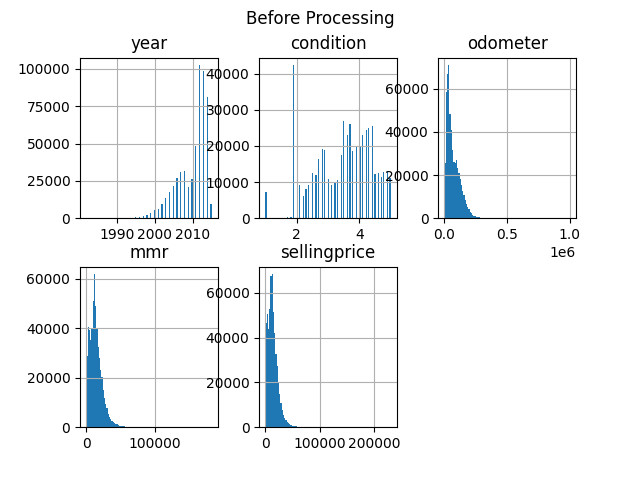
\includegraphics[width=.35\textwidth]{images/before_preprocessing.png}
    \caption{Graph of the numeric factors before processing}
    \label{fig:before_process}
\end{figure}
\begin{figure}[h]
    \centering
    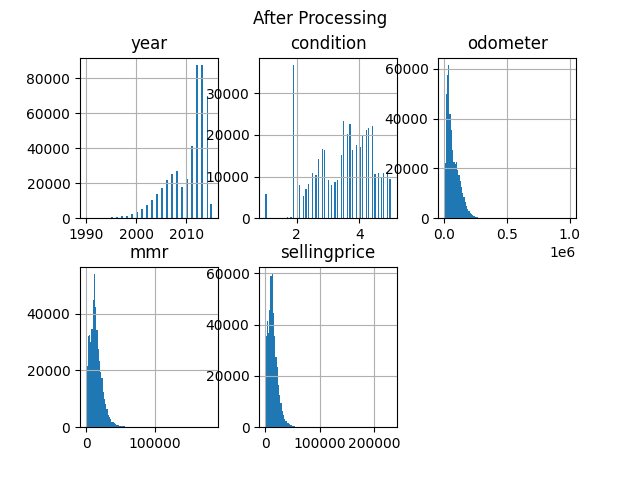
\includegraphics[width=.35\textwidth]{images/after_preprocessing.png}
    \caption{Graph of the numeric factors after processing}
    \label{fig:after_process}
\end{figure}
After removing all irrelevant factors, the categorized factors such as make, model, transmission, and color were encoded using OneHotEncoding. This allows each category in each factor to have a binary representation. At this point, the data was fully preprocessed, in a numeric format, and ready to be used in a model.
\subsection{Plotting}
From here, I had to learn which features had the most linear pattern when compared to the price of the vehicle. This could only be achieved by plotting each feature to the price and observing the shape.
\begin{figure}[h]
    \centering
    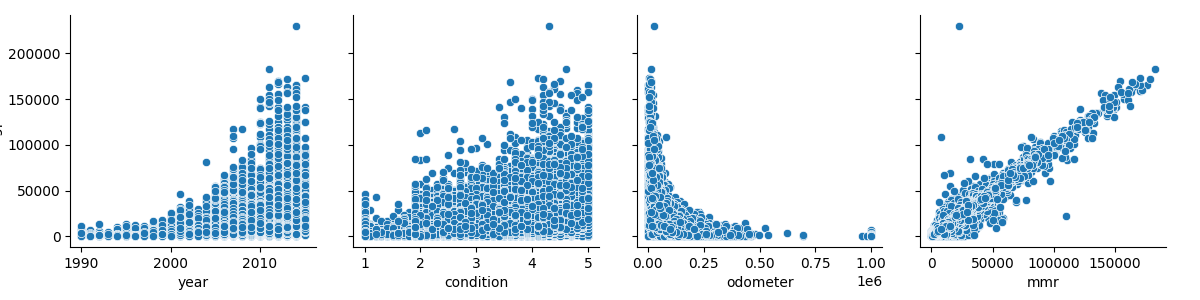
\includegraphics[width=.45\textwidth]{images/linearity.png}
    \caption{The vehicle's year, condition, odometer reading, and MMR (wholesale market value) mapped with the selling price}
    \label{fig:linearity}
\end{figure}
As shown in Figure \ref{fig:linearity}, there is a strong positive linear correlation between the MMR and the selling price, a weak positive linear correlation between the vehicle's year and condition again the selling price, and a strong negative correlation between the reading on the vehicle's odometer and selling price. These readings are backed up by a heatmap of these features in Figure \ref{fig:heat}, showing a strong positive correlation between the selling price and MMR, and a strong negative correlation between the selling price and the odometer reading.
\begin{figure}[h]
    \centering
    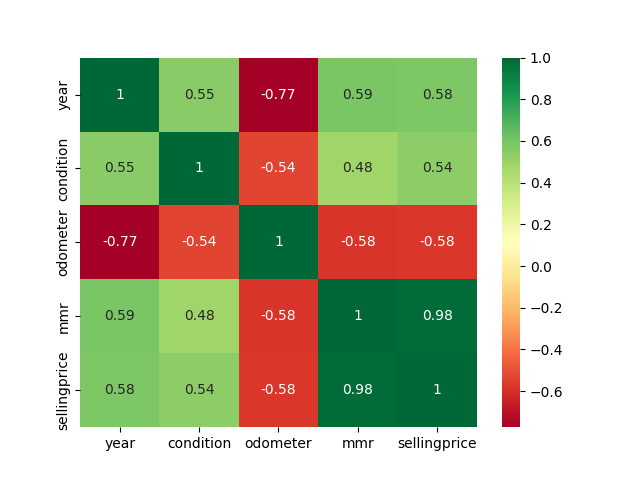
\includegraphics[width=.45\textwidth]{images/heatmap.png}
    \caption{Heatmap of the continuous features: Green = strong positive correlation, Red = strong negative correlation}
    \label{fig:heat}
\end{figure}
\subsection{Linear Regression Model}
Since there was such a strong linear connection between the continuous features and the price, I decided to first implement a linear regression model, as it is the easiest and quickest model to setup. It is a multiple linear regression model with 4 continuous features, 8 categorized features, and one dependant variable.
\subsection{Neural Network Model}
I also created a traditional ANN style neural network model, as I felt it had a good chance of providing a more accurate result than the linear regression model, albeit at the cost of a longer training time. The model uses two hidden layers of 125 and 25 nodes respectively. It takes the same input as the linear regression model.
%%%%%%%%%%%%%%%%%

\section{Experimental results (and technical correctness)}
\subsection{Experimental Environment}
Both of my models were written in Python using the pandas, sklearn, keras, tenserflow, and matplotlib libraries. All models were run on a computer with a 4 core, 3.5GHz CPU and 16GB of memory. The models were not GPU enhanced. In addition, the data split was 85\% training and 15\% testing.
\subsection{Neural Network Parameters}
The neural network model has two hidden layers of 125 and 25 nodes respectively. Each hidden layer uses the ReLu activation function with the final output later using a linear activation function. The model's compiler implements the Adam optimizer with a learning rate of 0.001. The model runs for 250 epochs at around 12,547 samples per epoch. The number of layers, the learning rate, and the number of epochs were all determined by training and comparing multiple different models through TenserBoard. The Mean Squared Error loss function was chosen to determine loss as it measures both variance and bias in the model.

As an added speed improvement, I implemented early stopping within the model that ends training when the loss does not improve over 10 consecutive epochs. If this is found, the weights from the epoch with the least loss are restored and returned as the result of the model.
\subsection{Results}
\begin{table}[h!]
\centering
\begin{tabular}{|l|l|l|}
\hline
                       & Linear Regression & Neural Network \\ \hline
$R^2$ Test Score     & 97.38\%           & 97.54\%        \\ \hline
$R^2$ Training Score & 97.45\%           & 97.55\%        \\ \hline
MSE Loss               & 2,362,095         & 2,265,596      \\ \hline
Training Time          & 3.64 minutes      & 38.52 minutes  \\ \hline
\end{tabular}
\caption{Results after training and testing both models}
\label{table:results}
\end{table}
As Table \ref{table:results} shows, both models resulted in highly similar $R^2$ scores for the testing data. In addition, both models have a similar Mean Squared Error loss. Therefore, these models are approximately 97\% accurate when given all required features. Also, the square root of the Mean Squared Error for each model is approximately 1,500. This verifies the effectiveness of the models because there is only about a 1,500 dollar difference between the true price of the car and the estimated price.

However, accuracy is not the only metric I measured. Both models took a drastically different amount of time to train. Linear regression only took around three and a half minutes while the neural network took 38 and a half minutes. Therefore, the linear regression model was faster by a factor of ten! Since both models resulted in similar accuracies, the linear regression model seems to be the better model of the two as it is much quicker to train.

When compared to the baseline model, the results are as expected.
\begin{figure}[h]
    \centering
    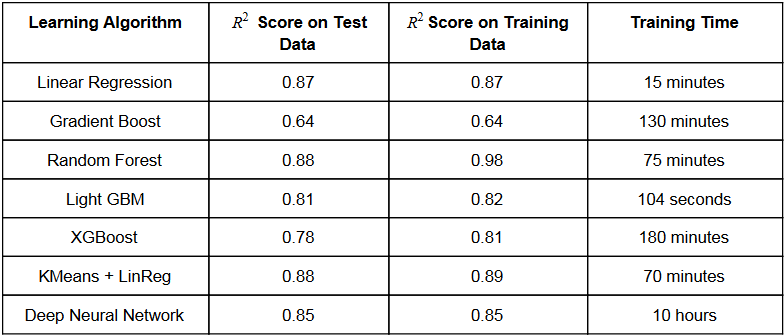
\includegraphics[width=.45\textwidth]{images/baseline_results.png}
    \caption{Results from the baseline project}
    \label{fig:base_result}
\end{figure}
As Figure \ref{fig:base_result} shows, the baseline's Linear Regression and Deep Neural Network models had similar accuracies while the Linear Regression model was much faster. However, compared to the baseline, this project's models are much more accurate. I believe this was due to the extra factors implemented in the dataset I used. They allowed for more flexability within the model to more accurately predict a used car's price.
%%%%%%%%%%%%%%%%%%%%

\section{Conclusion} 
Since both models were highly accurate, both would be acceptable to use when predicting used car prices. However, accuracy is not the only important factor when creating a model. As the linear regression model was ten times faster to train without any major accuracy penalties, the linear regression model stands as the best model to predict used car prices from a set of features in this circumstance. As both models stand now, I would prefer the linear regression model for the most accurate prediction in the least amount of time.
\subsection{Future Work}
In the future to improve this project, I would find a dataset with both more recent car listings and a larger feature set. Another viable addition would be to search and find accident claims based on a vehicle's VIN number. This would allow for another highly sought after feature. Finally, the neural network could certainly be optimized further, whether through adding more layers or through general tweaking. However, with an $R^2$ test accuracy of 97\%, the current model is certainly accurate enough for everyday use.

%%%%%%%%%%%%%%%%%%%%%%%
\bibliographystyle{IEEEtran}
\bibliography{References} % (15 - 25) references

\end{document}
